% !TEX root = ../main.tex
\chapter{Dashboard}
\label{ch:dashboard}

Since one of the goals of this thesis was to make these analyses available to a broader,
semi-technical audience, as described in~\ref{ch:goals},
a user-friendly streaming dashboard was created.
\\
This dashboard puts all the aforementioned theory into practice,
using the Twitter streaming API instead of data at rest,
as described in~\ref{subsec:dataAtRest-DataInMotion},
making it one of the most important chapters.

\section{Requirements}
\label{sec:requirement}

To make it easily accessible, it was decided to implement the dashboard as a web-based application.
Since it has to perform the analyses on streamed data from Twitter,
and the streaming API is rate limit in the number of connections that can be opened,
as described in~\ref{subsec:streaming},
each user needs to authenticate with a Twitter account.
That way, the application can scale with the number of users,
without the number of connection requests being limited by the application-rate-limit.
\\
A settings-dialog is required to enable the user to choose between any of the streams explained in~\ref{subsec:streaming},
and to configure all their respective parameters.
\\
To give the user a feeling for the stream he/she configured,
the 100 most recently streamed statuses are listed in a feed.
\\
Since the dashboard will not allow the user to train new models,
the best model for sentiment analysis, developed in~\ref{ch:sentimentAnalysis},
the best model for topic modeling, developed in~\ref{ch:topicModeling},
and the combination of both, developed in~\ref{ch:combiningSentimentAnalysisAndTopicModeling}
should be used to classify incoming statuses.
\\
The results of this classification should be visualized over time,
necessitating visualizations different to the previously used scatter plots, network graphs and pie charts.

\section{Architecture}
\label{sec:architecture}

The architecture of the dashboard is a simple client-server architecture.
To facilitate the analyses of the Twitter stream,
Kafka was used as a distributed messaging system as described in~\ref{subsec:kafka},
and Spark was used for distributed processing of the messages, as described in~\ref{subsec:spark}.
A simplified diagram of the architecture can be seen in~\ref{fig:architecture}.

\begin{figure}
    \centering
    \caption{Simplified diagram of the architecture}
    \label{fig:architecture}
    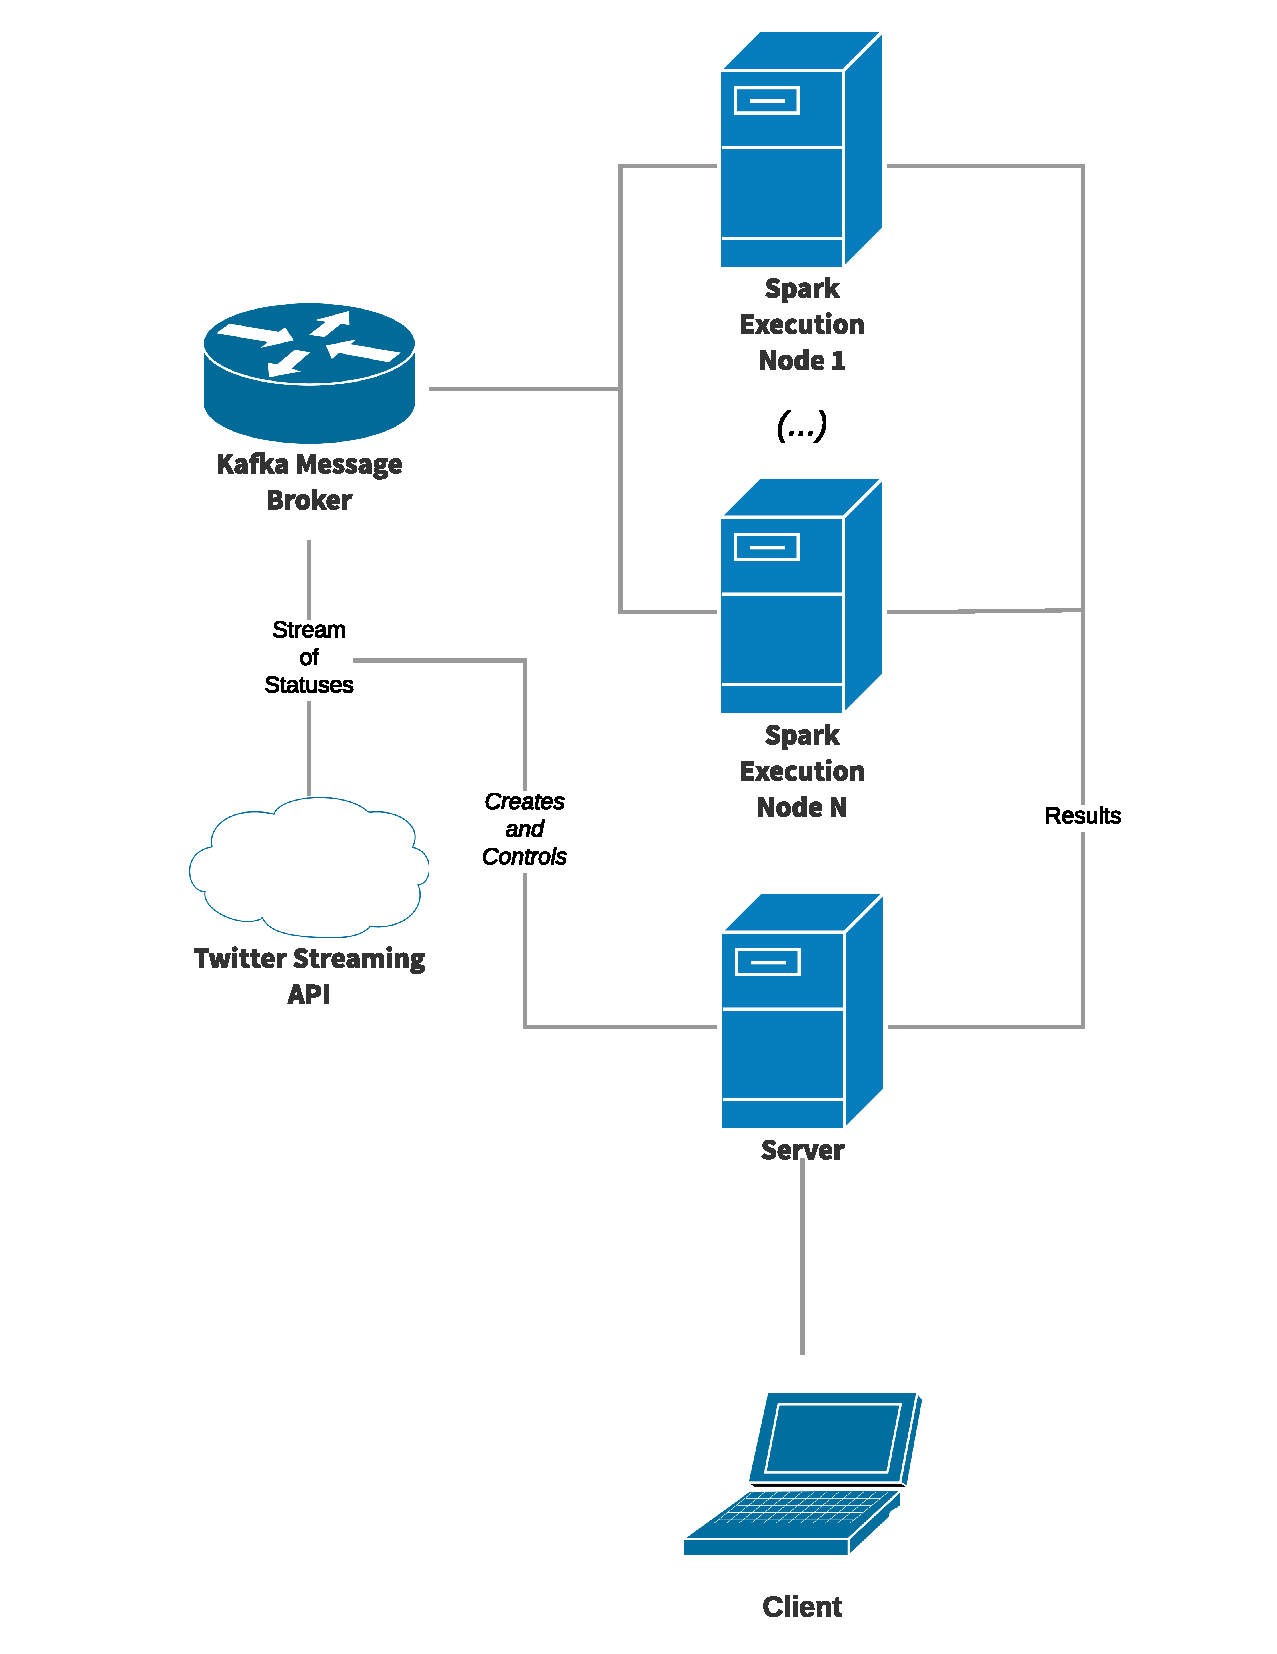
\includegraphics[width=10cm]{../figures/architecture.pdf}
\end{figure}

For the server, Flask~\cite{flaskDocs} was used, because it is written in Python and therefore works seamlessly with the rest of the code.
In the frontend, common web technologies such as HTML, CSS and JS were used, with Angular JS providing the framework~\cite{angularDocs}.
Furthermore, some miscellaneous technologies such as SCSS\cite{scssDocs} for more efficient styling and the taskrunner GruntJS~\cite{gruntDocs} for
minification, transpilation etc. were used.

\section{Dashboard Code Structure}
\label{sec:dashboardCodeStructure}

In the structure of the whole thesis explained
in~\ref{forest:dscookiecutter}, the dashboard application is located under \texttt{Thesis/src/visualization}.
This directory does not contain the code used for creating and analyzing the stream,
which, as described in~\ref{sec:projectStructure}, is located under \texttt{Thesis/streaming}.
On the first level, the structure is type-based, separating between client- and server-related code.
Since the type of asset (python-scripts for the server-related code, HTML/CSS/Javascript for the client-related code)
remains constant on every level below that, the structure is then switched to a feature-based one.
With this structure, full advantage can be taken of the modular nature of AngularJS~\cite{angularDocs}.
The structure of the dashboard-application part of the project can be seen in~\ref{forest:dashboard}.

\begin{figure}
    \caption{Structure of the dashboard-application part of the project under \texttt{Thesis/src/visualization}}
    \label{forest:dashboard}
    % @formatter:off
    \begin{forest}
        for tree={
            font=\footnotesize,
            grow'=0,
            child anchor=west,
            parent anchor=south,
            anchor=west,
            calign=first,
            inner xsep=7pt,
            edge path={
              \noexpand\path [draw, \forestoption{edge}]
              (!u.south west) +(7.5pt,0) |- (.child anchor) pic {folder} \forestoption{edge label};
            },
            before typesetting nodes={
              if n=1
                {insert before={[,phantom]}}
                {}
            },
            fit=band,
            before computing xy={l=15pt},
          }
        [visualization
          [dashboard \textit{contains client and server code for the dashboard application}
            [client
              [main \textit{The main (home) page}
              ]
              [main \textit{The actual dashboard}
              ]
            ]
            [server
              [api \textit{Facilitates interaction between the frontend and the stream}
              ]
              [auth \textit{All functionality for the authentication with Twitter}
              ]
            ]
          ]
        ]
    \end{forest}
    % @formatter:on
\end{figure}

\section{Implementation}
\label{sec:implementation}

Updating the settings was implemented as a HTML-form, styled with Bootstrap~\cite{bootstrapDocs},
which allows selecting which stream to analyze, and enables the user to modify all its parameters
described in the documentation~\cite{twitterDocs} and~\ref{subsec:streaming}.
A screenshot of the settings dialog of the dashboard can be seen in~\ref{fig:dashboard-settings}.

\begin{figure}
    \centering
    \caption{The settings dialog of the dashboard}
    \label{fig:dashboard-settings}
    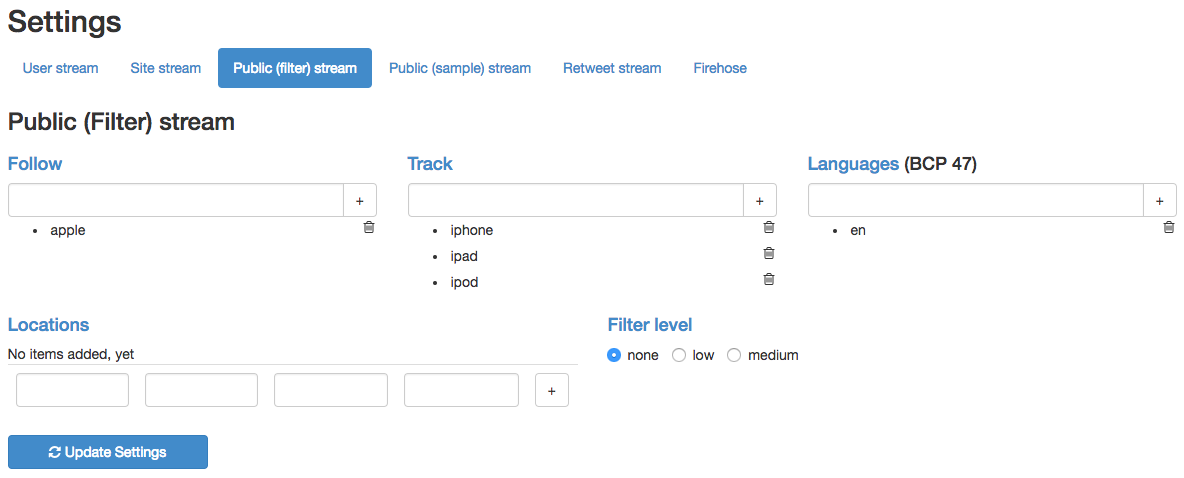
\includegraphics[width=\textwidth]{../images/dashboard_settings.png}
\end{figure}

When clicking the update-button, the current settings are sent to the server via a websocket,
which then closes the existing stream (if any), and opens a stream with the new settings.
\par
Incoming statuses are relayed into the Kafka messaging system described in~\ref{subsec:kafka}.
Kafka then distributes the statuses to the Spark execution nodes as described in~\ref{subsec:spark}.
\\
Preprocessing, tokenization, analyses and classifications were combined into one sparkjob.
This saves bandwidth, as some data like the dictionary might otherwise be transmitted to the same execution nodes twice,
since both sentiment analysis and topic modeling use it.
Also, this way, each status only needs to go through one execution node,
and the computational power required per status is still small enough for Kafka to distribute them efficiently.
Furthermore, this makes it easier to combine the results of sentiment analysis and topic modeling later on.
However, as explained in~\ref{subsec:nltk}, the NLTK is meant for teaching and research,
and the naive bayes classifier built with it did not meet the performance demands in a streaming scenario,
so an exact replica of the classifier was built using scikit~\cite{scikitDocs}, and was used instead.
The resulting function, applied on the incoming statuses on the execution nodes, can be seen in~\ref{fig:spark_job}

\begin{figure}
    \caption{The function used in the Spark job on incoming statuses}
    \label{fig:spark_job}
    % @formatter:off
    \begin{minted}{python}
    def analyze(element):
        # The actual tweet is the second element in a tupel
        tweet_str = element[1]
        # It's still a string, so parse it
        tweet = json.loads(tweet_str)
        # Just the text needed
        raw_text = tweet['text']
        # Using the same preprocessing function as everywhere else, for consistency
        text = preprocess(raw_text)
        # Use the same tokenization functions as everywhere else, for consistency...
        # ...without stopword removal for sentiment classification
        tokens_sa = sa_tokenize(text)
        # ... with stopword removal for topic modeling
        tokens_lda = lda_tokenize(text)

        # The update should contain...
        update = dict()
        # ...the sentiment...
        update['sentiment'] = analyze_sentiment(tokens_sa)
        # ...the topics...
        update['topics'] = model_topics(tokens_lda)
        # ...and the tweet itself (or at least what we need from it in the frontend).
        update['tweet'] = {
            'text': raw_text,
            'user': {
                'name': tweet['user']['name']
            }
        }

        return update
    \end{minted}
    % @formatter:on
\end{figure}

The update containing the results and the tweet itself is then sent to the master node,
which is also the server, as seen in~\ref{fig:architecture}.
The server then sends it to the client via a websocket.
\par
The client keeps a FIFO-queue of all incoming updates, facilitating a sliding window of the analysed statuses.
This way, a moving average can be calculated on the values, which represents the overall, \textit{average},
sentiment and topics on the stream, without too much delay.
The size of this queue, or \textit{window size}, has to be chosen carefully to reduce noise without suppressing actual signals.
A good window size was found to be \texttt{200}.
As described in~\ref{sec:requirement}, the visualizations needed to be changed to incorporate a timeline.
To visualize changes in the incoming statuses live, the results were plotted in a continually moving line chart over time.
The library Smoothie Chart~\cite{smoothieDocs} was used to implement these charts.
For all of these charts, one vertical section represents one second.

\section{Testing}
\label{sec:testing}

For testing, the filter stream was used,
the language was set to english (since our models are trained on english data only),
and only one keyword was tracked.
\par
First, the keyword was set to\texttt{iPhone},
and the stream was left running until the queue was filled and all results calculated from fewer elements
(which might look noisy) were no longer visible on the timeline.
Then, to artificially provoke a change in sentiment,
the streaming settings were updated to only track the keyword \texttt{people} without resetting the charts or the queue (and therefore the moving average).
This illustrates what a sudden change in sentiment for a stream would look like if it were observed naturally.
The resulting graph, and the associated values, can be seen in~\ref{fig:dashboard-sentiment}

\begin{figure}
    \centering
    \caption{The sentiment chart plus values, showing the change in sentiment after changing the stream settings}
    \label{fig:dashboard-sentiment}
    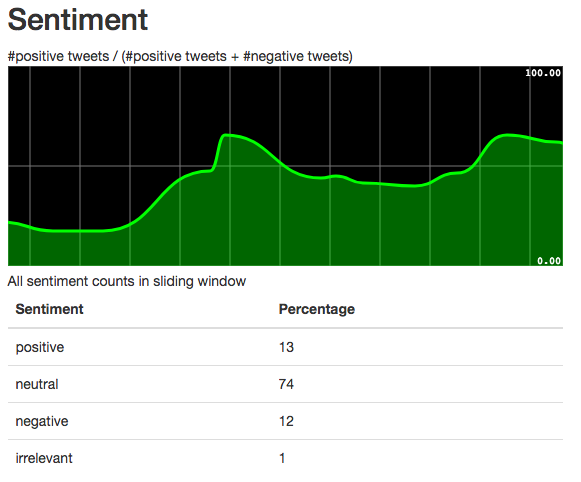
\includegraphics[\textwidth]{../images/dashboard_sentiment.png}
\end{figure}

\par
After running the stream with these settings for a while, a natural change in topics was observed, which can be seen in~\ref{fig:dashboard-topics}.
Even though the keyword was still \texttt{people}, and the dominating topic was, as expected, topic number 5,
for which this keyword is one of the most likely ones, the prevalence of this topic decreased in favor of topics 4 and 9,
indicating a wave of tweets associated with these topics occurring at that moment.
These events were observed regularly, and might even indicate bot activity~\cite{chu2012detecting}.

\begin{figure}
    \centering
    \caption{The topics chart plus values, showing the naturally occuring change in topic distribution}
    \label{fig:dashboard-topics}
    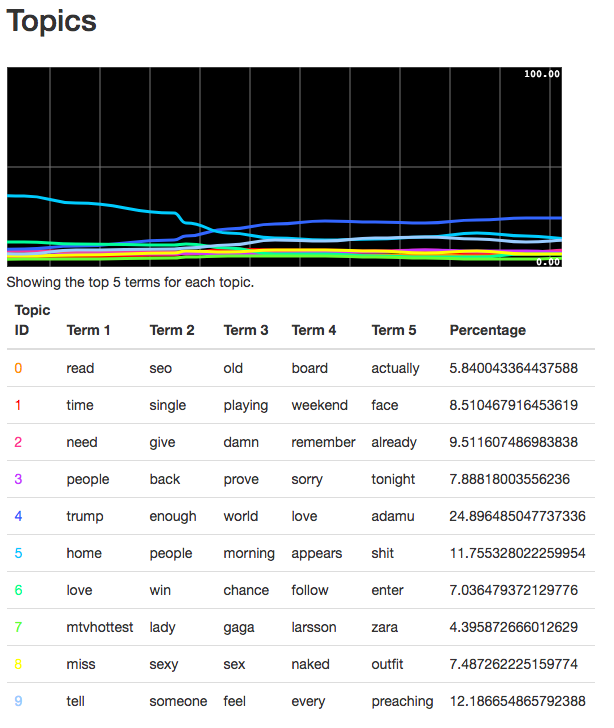
\includegraphics[\textwidth]{../images/dashboard_topics.png}
\end{figure}

\par
To calculate the sentiment by topic for the combination-visualization,
the sliding window was set to 1000, since topics with little prevalence and few opinionated statuses
(those that are labeled positive or negative) would give very noisy results otherwise.
That window size was found to give the right balance between reducing noise and not suppressing any signal.
\par
Even though the sentiments by topic were mostly free of noise, they did not converge,
indicating that some topics have an inherently different sentiment.
\par
As with the visualization of sentiment,
the settings were changed from tracking \texttt{apple} to tracking \texttt{weekend}, to illustrate a change in sentiment by topic.
This still gave interesting results, showing that depending on which keywords the stream is tracking,
the sentiment per topic differs.
The resulting graph and associated values can be seen in~\ref{fig:dashboard-sentiment-by-topic}.

\begin{figure}
    \centering
    \caption{The sentiment by topic chart plus values, showing the change in sentiment by topic after changing the stream settings}
    \label{fig:dashboard-sentiment-by-topic}
    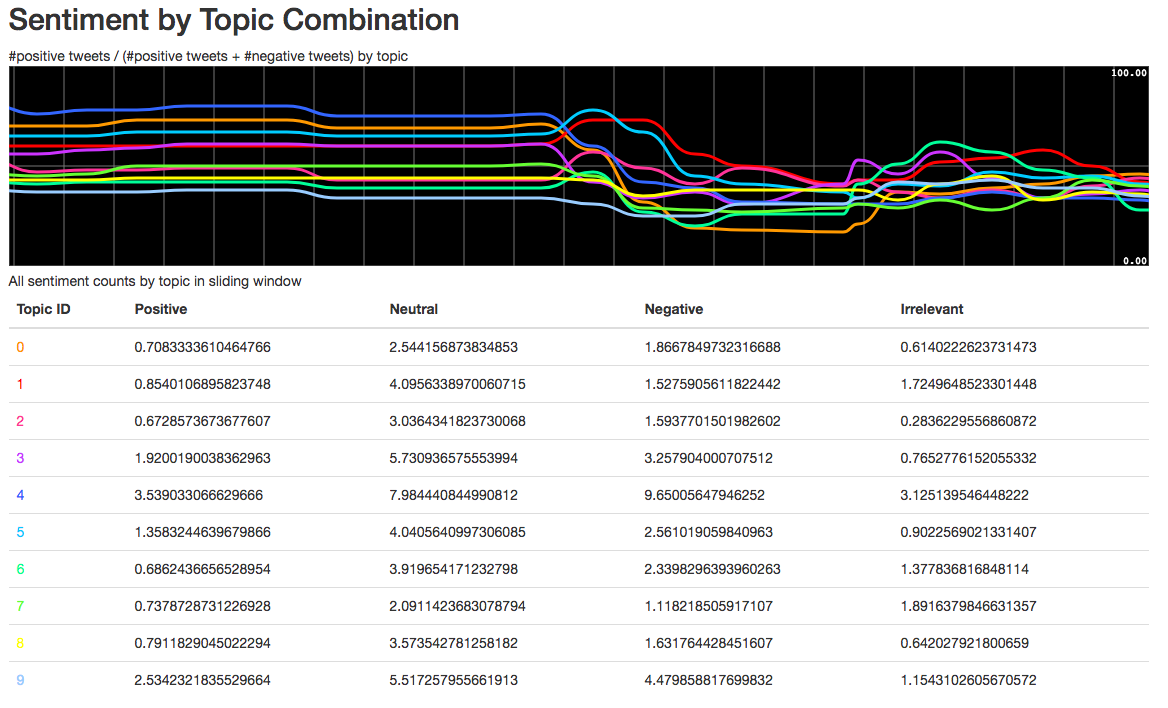
\includegraphics[\textwidth]{../images/dashboard_sentiment_by_topic.png}
\end{figure}

The part of the dashboard showing actual statuses coming in to give the user a feeling for the stream is not shown here due to Twitter's TOS.